%--------------------------------------------------------------------------------
\chapter{Mesh treatment}
%--------------------------------------------------------------------------------
When the mesh file is being treated, the computation parameters given by the
user help \stbtel to initiate the followong operations:
\begin{itemize}
\item Read of the mesh file and of the connectivity table
\item Mesh extraction (if required by the user)
\item Print of the geometric data on the listing printout
\item Cutting elements in four (if required by the user)
\item Dry elements elimination (if required by the user)
\item The mesh is initialised on the \telemacsystem format (\stbtel check
especially that the local numeration of the nodes is done on the trigonometric
way).
\item Analysis of the boundaries (area outline, islands) and building of the
boundary points table
\item Overstressed elements elimination (if required by the user)
\item Re-numbering of the nodes used for the optimisation of the matrix storage
on the \telemac{2} software (if required by the user)
\item Elimination of backward dependencies (if required by the user)
\item Interpolation of the bathymetry on the mesh
\item Building of the geometry file
\item Building of the boundary conditions file
\end{itemize}

%--------------------------------------------------------------------------------
\section{Initial treatment}
%--------------------------------------------------------------------------------
\stbtel first goal is to read a mesh file that comes from an outer software. In
this case, the user must indicate the name of the file to be read with the
keyword \telkey{UNIVERSAL FILE}, and, with the keyword \telkey{MESH GENERATOR},
indicates also the name of the software used for mesh generation. This keyword
can be selected among the following:
\begin{itemize}
\item SUPERTAB6 (version 6 of  SUPERTAB mesh generator)
\item SUPERTAB4 (version 4 of  SUPERTAB mesh generator)
\item MASTER2 (version 2 of the MASTER-SERIES mesh generator)
\item SIMAIL,
\item SELAFIN
\item TRIGRID,
\item FASTTABS.
\end{itemize}
When using TRIGRID, the file containing the connectivity table (file with a
“triangle” format) must be given through the keyword \telkey{MESH ADDITIONAL
DATA FILE}.\\
Within a mesh, the three nodes of some triangles can be boundary nodes. In this
case, the computation codes can generate wrong results. This type of elements
called overstressed triangles, must be eliminated when the mesh is being
treated. This action is done with the logical keyword \telkey{OVERSTRESSED
TRIANGLES CUTTING} and which the default value in NO. This action is done
by \stbtel.\\
It adds a point at the inertia center of the triangle, in order to
create three more elements. Sometimes, this action can generate flat triangles.
In this case, \stbtel can take the decision to swap segments, in clear, to
reverse the cutting of a quadrangle on the other diagonal. (see Figure
\ref{fig:stress} below). A balance sheet of the overstressed elements
elimination is drawn up with the listing printout.

\begin{figure}[H]%
\begin{center}
%
  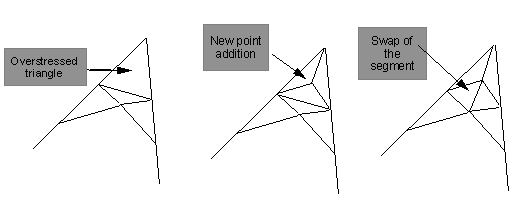
\includegraphics[width=0.9\textwidth]{./graphics/stress}
%
\end{center}
\caption
{Overstressed triangles elimination.}
\label{fig:stress}
\end{figure}


When the mesh is treated, \stbtel allows the elimination of the points that
have a distance value lower at a special value. The user must indicate this
value with the keyword \telkey{MINIMUM DISTANCE BETWEEN TWO POINTS}. This
default value is 0 (no elimination). If the value indicated by the user
eliminates lots of points, \stbtel could be not able to re-build the mesh. In
this case, the computation is automatically interrupted.

%--------------------------------------------------------------------------------
\section{Boundary conditions treatment}
%--------------------------------------------------------------------------------
when a mesh is treated, \stbtel generates automatically the boundary conditions
file.\\
With TRIGRID and SUPERTAB, a colour code stored on the mesh file and associated
with each boundary point permits \stbtel to define the codes to  be generated
within the boundary conditions file (see annexe 10).\\
With FASTTABS, the boundary conditions type can be supply in an additional
file. The user must give the name of this file with the keyword \telkey{MESH
ADDITIONAL DATA FILE} and activate the logical keyword \telkey{BOUNDARY
CONDITIONS IN THE ADDITIONAL FILE}.\\
Then, when using a mesh from SIMAIL software, or from a Selafin file, \stbtel
does not have any information about the type of the boundary conditions. The
generated file assigns with the code “solid boundary” to all the boundary
points.

%--------------------------------------------------------------------------------
\section{Mesh extraction}
%--------------------------------------------------------------------------------
With \stbtel, it is possible to extract a sub-mesh from a global mesh. To
extract one, first of all, the user must choose the polygon that will define
the area of the mesh to be extracted (in the anti clockwise order). This
polygon must have a convex shape.\\
The number of vertices of this polygon must be indicated with the keyword
\telkey{NUMBER OF VERTICES OF THE POLYGON TO EXTRACT THE MESH} and the
coordinates of the points with the keywords \telkey{ABSCISSSAE OF THE VERTICES
OF THE POLYGON TO EXTRACT THE MESH} and  \telkey{ORDINATES OF THE VERTICES OF
THE POLYGON TO EXTRACT THE MESH}.\\
When the mesh is extracted, the user can project new boundaries nodes on the
polygon segments. This action is activated with the logical keyword
\telkey{PROJECTION AFTER EXTRACTION}, with a default value NO.
%--------------------------------------------------------------------------------
\section{Refinement}
%--------------------------------------------------------------------------------
When using \stbtel, a mesh can be refine inside of a zone. To use it, the user
must choose the polygon that will define the area to be refined. As for a mesh
to be extracted, this polygon must have a convex shape and the vertices must be
given with an anti clock wise order. The refinement  generated re-cut the
triangles in four.\\
For the user, the actions to be done are the same than the one used to extract
a mesh.  The number of the vertices of the polygon is given with the keyword
\telkey{NUMBER OF THE VERTICES OF THE POLYGON TO REFINE THE MESH} and the
coordinates of the points with the keyword \telkey{ABSCISSAE OF THE VERTICES OF
THE POLYGON TO REFINE THE MESH} and \telkey{ORDINATES OF THE VERTICES OF THE
POLYGON TO REFINE THE MESH}.
%--------------------------------------------------------------------------------
\section{Special treatments}
%--------------------------------------------------------------------------------
With \stbtel, it is possible to refine the mesh in bulk. This action generates
a new point in the middle of each segments of the triangles. Therefore, each
initial element is cut into four new elements. This action is done with the the
logical keyword \telkey{CUTTING TRIANGLES IN FOUR}, which default value is NO.\\
When using the simulation codes on a vector computer, it is necessary to
foresee the elimination of backward dependencies. This action is done with the
keyword \telkey{ELIMINATION OF THE BACKWARD DEPENDENCIES} and indicates the
length of the vector with the keyword \telkey{VECTOR LENGTH}, with a default
value 1, which means a scalar machine.\\
At least, the use of the assembled elementary storage method for the matrix
storage in \telemac{2} requires a special point numbering that could be done by
\stbtel. This action is completed with the logical keyword \telkey{NODES
RENUMBERING} (default value NO).
